\section{Durchführung und Aufbau}
\label{sec:Durchführung}

\begin{figure}[h]
  \centering
  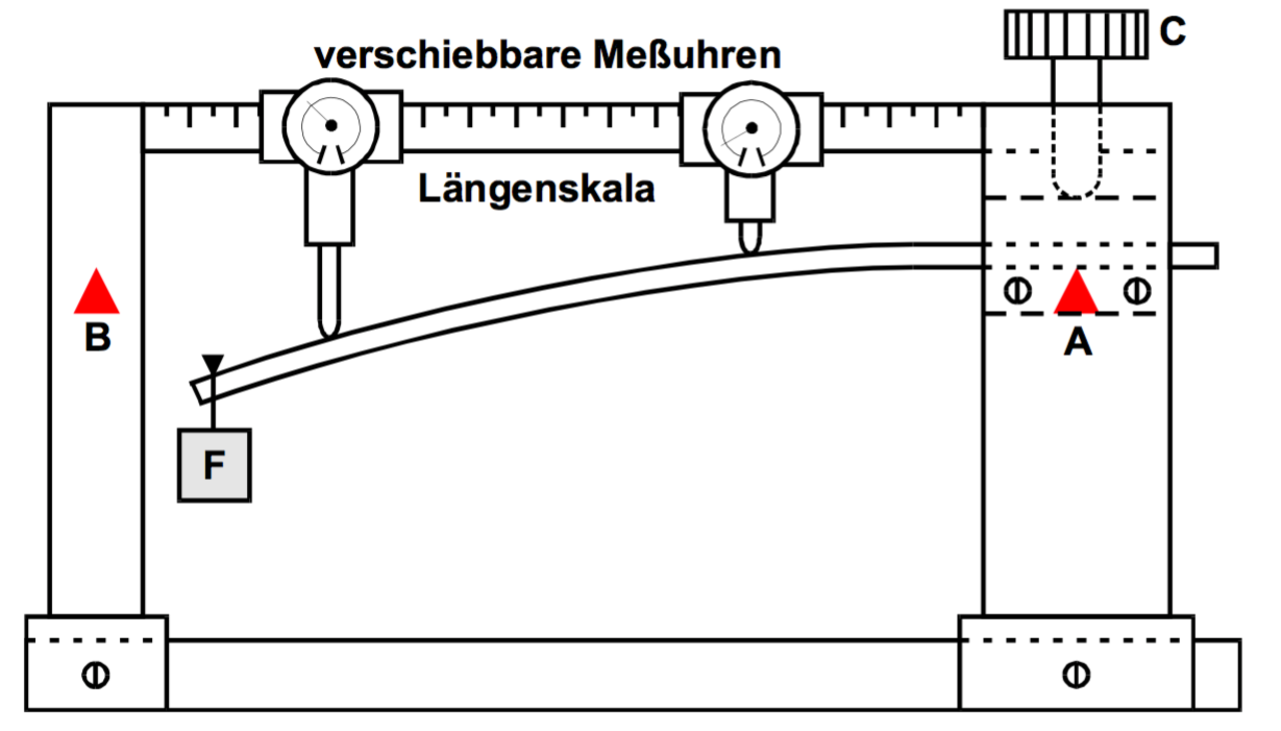
\includegraphics[width = \textwidth]{pics/aufbaueinseit.pdf}
  \caption{Apparatur zur Vermessung elastisch gebogener Stäbe\cite{anleitung}.}
  \label{fig:aufbau}
\end{figure}

In Abbildung \ref{fig:aufbau} ist eine schematische Darstellung der zu
verwendenden Apparatur zu sehen. Hier kann ein Gewicht F an den Stab gehängt
werden und der Stab kann entweder mit der Vorrichtung C eingespannt werden oder
an den Punkten A und B aufgelegt werden. Die beiden Messuhren sind auf einer
Längenskala verschiebbar.

\begin{itemize}
  \item Um später den berechneten Elastizitätsmodul mit Literaturwerten zu
  vergleichen muss zunächst das Material benannt werden.
  Dazu wird die Dichte bestimmt. Zu diesem Zweck wird die Länge sowie der
  Durchmesser zehn Mal vermessen; außerdem wird die Masse ein Mal bestimmt.
  Mehrfache Messungen dienen der Genauigkeit.
  Diese Messungen werden bei einem ausgewählten Stab kreisförmigen
  Querschnitts sowie bei einem mit quadratischem Querschnitt durchgeführt.

  \item Nun wird die Biegung bei einseitiger Einspannung mit beiden
  Stäben durchgeführt. Dazu wird der jeweilige Stab an einer Seite mit der
  Vorrichtung C eingespannt. Das Gewicht, das den Stab an der anderen
  Seite belastet, wird so gewählt, dass die maximale Durchbiegung zwischen
  3 und \SI{7}{\milli\meter} liegt.
  Dann werden 30 Messwertpaare aus Durchbiegung $D(x)$ und Position $x$ der Messuhr
  aufgenommen. Die Durchbiegung $D(x)$ ist die Differenz zwischen
  Durchbiegung mit Gewicht $D_{\g{M}}$ und ohne Gewicht $D_0(x)$.

  \begin{equation*}
    D(x) = D_{\g{M}} - D_0(x)
  \end{equation*}

  Gemessen wird in Nähe des Gewichts genauer, wobei immer größere Abstände
  genommen werden desto weiter sich die Messuhr von dem Gewicht entfernt.
  Darüber hinaus wird die Länge des Stabs von Einspannung bis zu dem
  Gewicht drei Mal gemessen. Das angehängte Gewicht wird ein Mal gemessen.

  \item Zuletzt wird die Durchbiegung bei beidseitiger Auflage vermessen.
  Der Stab wird links und rechts aufgelegt und das Gewicht wird in der Mitte
  angehängt. Dazu wird ein Gewicht sehr großer Masse gewählt. Die Länge
  von Auflage zu Auflage wird ein Mal gemessen und der Mittelpunkt
  bestimmt. Dann wird links und rechts von dem Gewicht jeweils 15 Mal
  die Durchbiegung $D(x)$, wie oben beschrieben, gemessen. Erneut ist
  die Genauigkeit um das Gewicht herum größer.


\end{itemize}
